\documentclass[12pt]{article}
\usepackage[letterpaper,margin=15mm,top=18mm,bottom=18mm,headheight=15pt,headsep=5mm,footskip=10mm]{geometry}
\usepackage[T1]{fontenc}
\usepackage{helvet}
\renewcommand{\familydefault}{\sfdefault}
\usepackage{tikz}
\usetikzlibrary{arrows.meta,calc}
\usepackage{fancyhdr}
\usepackage{array}
\usepackage{xcolor}
\definecolor{redgood}{RGB}{185,63,68}
\definecolor{bluegood}{RGB}{41,107,164}
\definecolor{pale}{RGB}{243,244,245}
\definecolor{ink}{RGB}{30,35,40}
\color{ink}
\setlength{\parindent}{0pt}
\setlength{\parskip}{3.5mm}
\renewenvironment{center}{\par\vspace{1mm}\centering}{\par\vspace{1mm}}
\pagestyle{fancy}
\fancyhf{}
\renewcommand{\headrulewidth}{0pt}
\renewcommand{\footrulewidth}{0pt}
\fancyhead[L]{\small Week 58 / Fair division / \Band}
\fancyfoot[L]{\scriptsize Bellingham Math Circle / Week 58 / W58-\Packet-v2}
\fancyfoot[R]{\scriptsize\thepage}
\newcommand{\Band}{Grades 2--5}
\newcommand{\Packet}{shared}
\newcommand{\newband}[1]{\newpage\renewcommand{\Band}{#1}}
\newcommand{\prob}[2]{\noindent\textbf{Problem #1:} #2\par}
\newcommand{\good}[4]{% x y type label, in mm
  \ifnum#3=1\def\gc{redgood}\fi
  \ifnum#3=2\def\gc{bluegood}\fi
  \draw[rounded corners=1mm,fill=white,draw=ink,line width=.6pt] (#1,#2) rectangle ++(25,25);
  \ifnum#3=1\draw[fill=\gc,draw=\gc] (#1+12.5,#2+15.5) circle (4.2mm);\fi
  \ifnum#3=2\draw[fill=\gc,draw=\gc] (#1+8.3,#2+11.3) rectangle ++(8.4,8.4);\fi
  \node[font=\small] at (#1+12.5,#2+5) {#4};
}
\newcommand{\smallgood}[4]{% x y type label, mm
  \ifnum#3=1\def\gc{redgood}\fi
  \ifnum#3=2\def\gc{bluegood}\fi
  \draw[rounded corners=.8mm,fill=white,draw=ink,line width=.5pt] (#1,#2) rectangle ++(14,17);
  \ifnum#3=1\draw[fill=\gc,draw=\gc] (#1+7,#2+11) circle (2.6mm);\fi
  \ifnum#3=2\draw[fill=\gc,draw=\gc] (#1+4.4,#2+8.4) rectangle ++(5.2,5.2);\fi
  \node[font=\scriptsize] at (#1+7,#2+3) {#4};
}
\newcommand{\valuedots}[3]{% x y count
  \ifnum#3>0\foreach \i in {1,...,#3}{\fill[ink] (#1+4*\i,#2) circle (1.1mm);}\fi
}
\newcommand{\linearea}[1]{\vspace{1mm}\foreach \i in {1,...,#1}{\noindent\rule{\linewidth}{.25pt}\par\vspace{8mm}}}
\newcommand{\trayrecord}[2]{% x y
  \draw[rounded corners=2mm,draw=black!45,line width=.7pt] (#1,#2) rectangle ++(82,26);
  \node[anchor=north west,font=\small] at (#1+3,#2+24){A};
  \draw[black!25] (#1+41,#2+2) -- (#1+41,#2+24);
  \node[anchor=north west,font=\small] at (#1+44,#2+24){B};
}
\newcommand{\prefmini}{
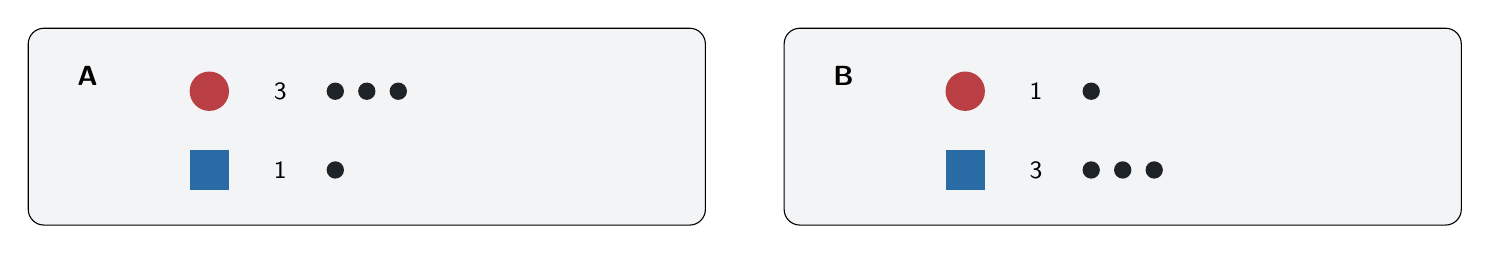
\begin{tikzpicture}[x=1mm,y=1mm]
  \foreach \x/\name/\r/\b in {0/A/3/1,96/B/1/3}{
    \draw[rounded corners=2mm,fill=pale] (\x,0) rectangle ++(86,25);
    \node[anchor=west,font=\bfseries] at (\x+5,19){\name};
    \fill[redgood] (\x+23,17) circle (2.5mm);
    \node[font=\small] at (\x+32,17){\r};
    \valuedots{\x+35}{17}{\r}
    \fill[bluegood] (\x+20.5,4.5) rectangle ++(5,5);
    \node[font=\small] at (\x+32,7){\b};
    \valuedots{\x+35}{7}{\b}
  }
\end{tikzpicture}}
\newcommand{\strip}[2]{% x y: schematic 180x24
  \draw[fill=redgood!22] (#1,#2) rectangle ++(90,24);
  \draw[fill=bluegood!22] (#1+90,#2) rectangle ++(90,24);
  \draw (#1,#2) rectangle ++(180,24);
  \draw (#1+90,#2) -- ++(0,24);
  \node[font=\small] at (#1+45,#2+12){red: 150 mm};
  \node[font=\small] at (#1+135,#2+12){blue: 150 mm};
}
\newcommand{\checkbar}[2]{
  \draw[line width=.8pt] (#1,#2) -- ++(100,0);
  \draw[line width=.8pt] (#1,#2-2) -- ++(0,4);
  \draw[line width=.8pt] (#1+100,#2-2) -- ++(0,4);
  \node[font=\small,anchor=south] at (#1+50,#2+2){100 mm};
}

\begin{document}

Keep each person's preference card unchanged during a trial. A tray's value is the sum of its cards' values, using the same person's preferences for every tray. Use every card once. Cards stay whole unless the problem allows cutting. Ties are allowed.

\begin{center}
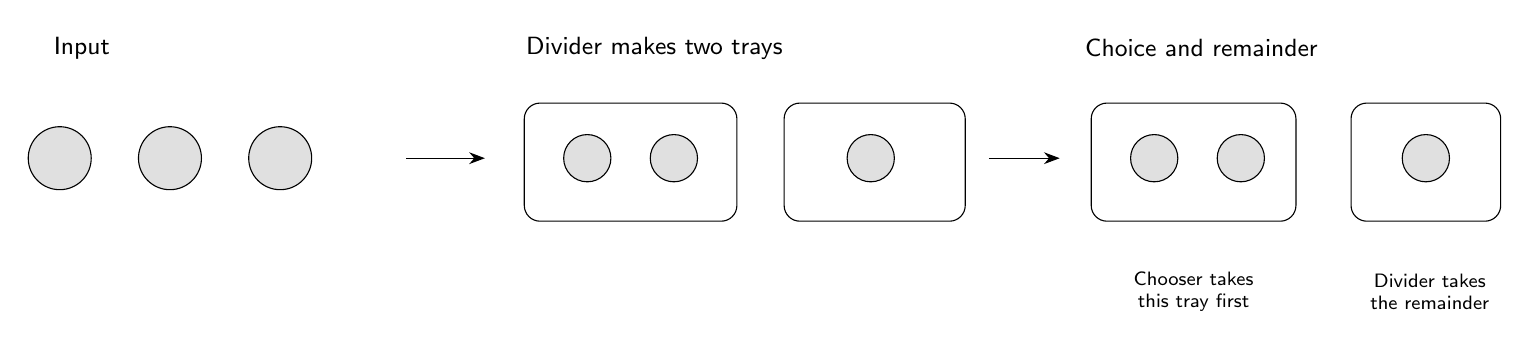
\begin{tikzpicture}[x=1mm,y=1mm]
  \node[anchor=west,font=\small] at (0,39){Input};
  \node[anchor=west,font=\small] at (60,39){Divider makes two trays};
  \node[anchor=west,font=\small] at (131,39){Choice and remainder};
  \foreach \x in {2,16,30}{\draw[fill=black!12] (\x,25) circle (4mm);}
  \draw[-{Stealth[length=2mm]}] (46,25) -- (56,25);
  \draw[rounded corners=2mm] (61,17) rectangle (88,32);
  \draw[rounded corners=2mm] (94,17) rectangle (117,32);
  \foreach \x in {69,80}{\draw[fill=black!12] (\x,25) circle (3mm);}
  \draw[fill=black!12] (105,25) circle (3mm);
  \draw[-{Stealth[length=2mm]}] (120,25) -- (129,25);
  \draw[rounded corners=2mm] (133,17) rectangle (159,32);
  \draw[rounded corners=2mm] (166,17) rectangle (185,32);
  \foreach \x in {141,152}{\draw[fill=black!12] (\x,25) circle (3mm);}
  \draw[fill=black!12] (175.5,25) circle (3mm);
  \node[font=\scriptsize,align=center] at (146,8){Chooser takes\\this tray first};
  \node[font=\scriptsize,align=center] at (176,8){Divider takes\\the remainder};
\end{tikzpicture}
\end{center}

\prob{1}{Use preference cards A and B. Divide these cards into two trays; your partner chooses a tray first, and you take the remainder. Find divisions where both people would keep their tray instead of trading. Swap who divides.}

\begin{center}\prefmini\end{center}
\begin{center}
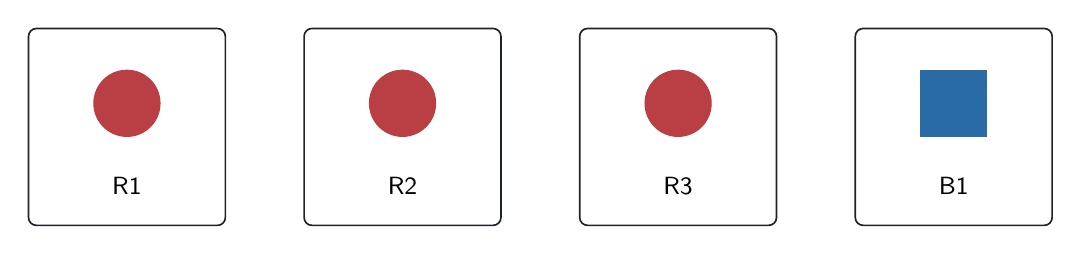
\begin{tikzpicture}[x=1mm,y=1mm]
  \good{20}{0}{1}{R1}\good{55}{0}{1}{R2}\good{90}{0}{1}{R3}\good{125}{0}{2}{B1}
\end{tikzpicture}
\end{center}
\begin{center}
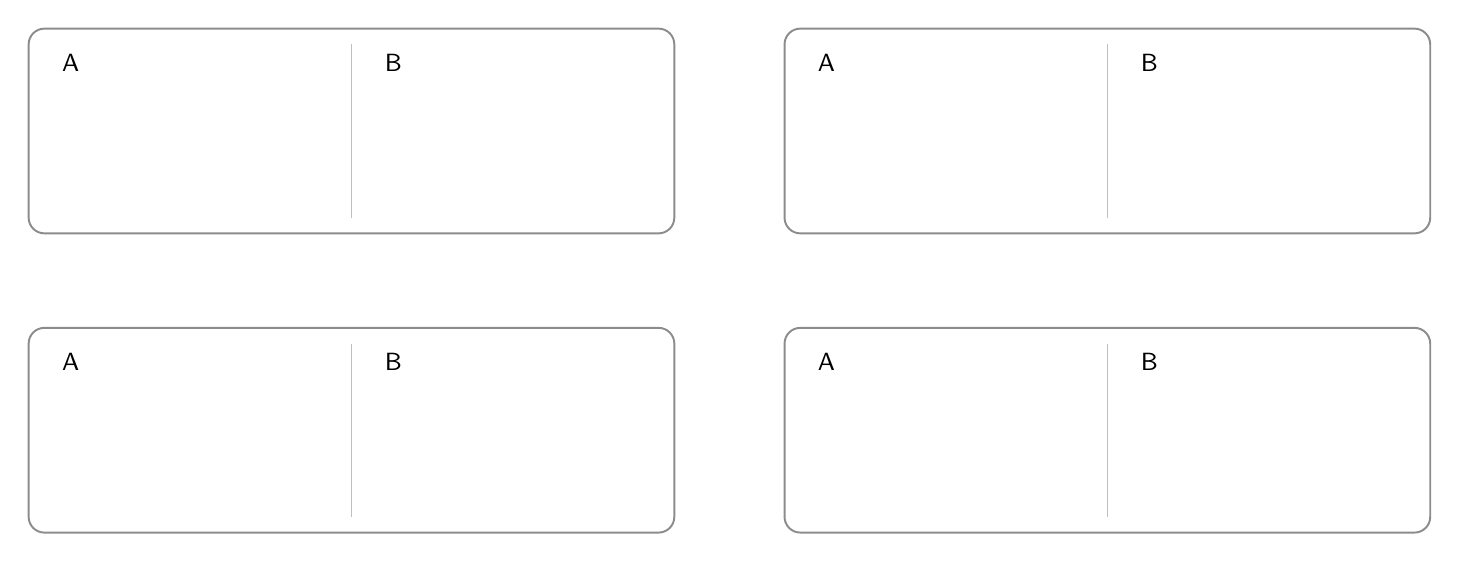
\begin{tikzpicture}[x=1mm,y=1mm]
  \trayrecord{0}{38}\trayrecord{96}{38}
  \trayrecord{0}{0}\trayrecord{96}{0}
\end{tikzpicture}
\end{center}

\newband{Grades 2--5}
For each person, a division is \emph{envy-free} when their own tray is worth at least as much as the other tray. It is \emph{proportional} when their own tray is worth at least half of all the cards. Use that person's preferences for each check.

\prob{2}{Use A and B's preference cards with R1, R2, B1 and B2. Find every complete division that is envy-free for both people. Which of your divisions are proportional for both people? Different card labels count as different cards.}

\begin{center}\prefmini\end{center}
\begin{center}
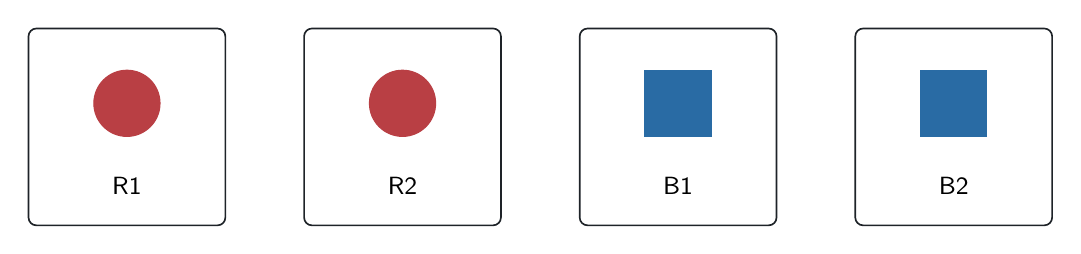
\begin{tikzpicture}[x=1mm,y=1mm]
  \good{20}{0}{1}{R1}\good{55}{0}{1}{R2}\good{90}{0}{2}{B1}\good{125}{0}{2}{B2}
\end{tikzpicture}
\end{center}
\begin{center}
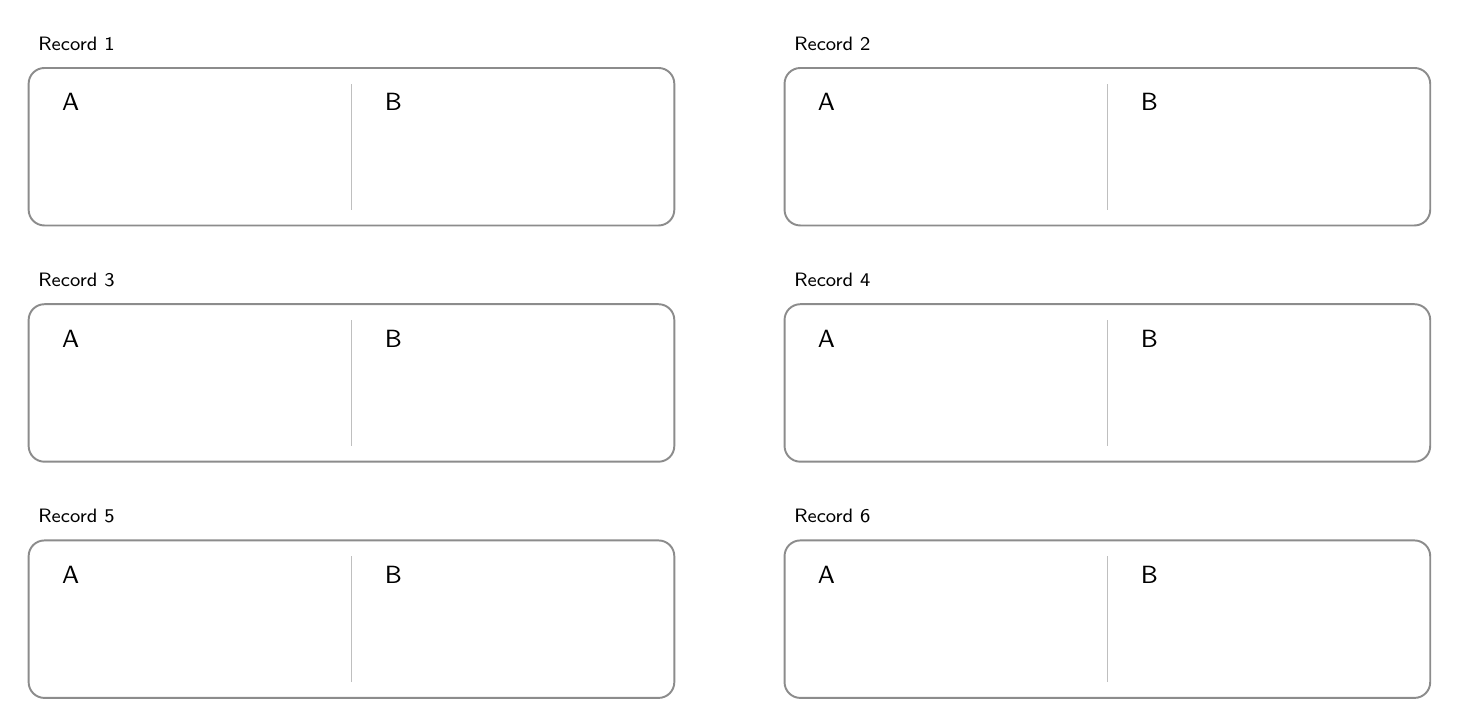
\begin{tikzpicture}[x=1mm,y=1mm]
  \foreach \x/\y/\n in {0/60/1,96/60/2,0/30/3,96/30/4,0/0/5,96/0/6}{
    \node[anchor=south west,font=\scriptsize] at (\x,\y+21){Record \n};
    \draw[rounded corners=2mm,draw=black!45,line width=.7pt] (\x,\y) rectangle ++(82,20);
    \node[anchor=north west,font=\small] at (\x+3,\y+18){A};
    \draw[black!25] (\x+41,\y+2) -- (\x+41,\y+18);
    \node[anchor=north west,font=\small] at (\x+44,\y+18){B};
  }
\end{tikzpicture}
\end{center}
\begin{center}
\renewcommand{\arraystretch}{1.6}
\begin{tabular}{|p{25mm}|p{33mm}|p{33mm}|p{33mm}|p{28mm}|}
\hline
\multicolumn{5}{|l|}{Saved division: Record \rule{12mm}{.25pt}}\\\hline
Observer & Their own tray & The other tray & All four cards & Half of all four\\\hline
A & & & &\\\hline
B & & & &\\\hline
\end{tabular}
\end{center}

\newband{Grades 2--5}
On a paper strip, the numbers on A and B's preference cards give the value of a whole 150 mm color panel. Within one color, value follows length: half a panel has half its value.

\begin{center}
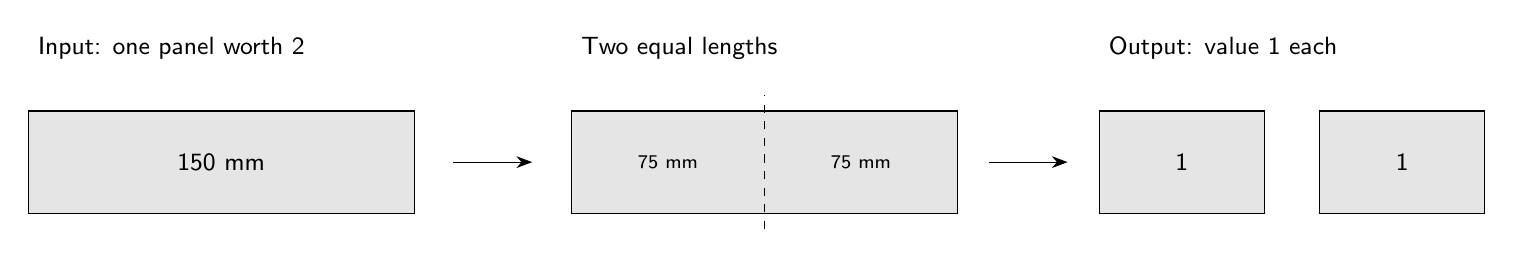
\begin{tikzpicture}[x=1mm,y=1mm]
  \node[anchor=west,font=\small] at (0,31){Input: one panel worth 2};
  \draw[fill=black!10] (0,10) rectangle (49,23);
  \node[font=\small] at (24.5,16.5){150 mm};
  \draw[-{Stealth[length=2mm]}] (54,16.5) -- (64,16.5);
  \node[anchor=west,font=\small] at (69,31){Two equal lengths};
  \draw[fill=black!10] (69,10) rectangle (118,23);
  \draw[dashed] (93.5,8) -- (93.5,25);
  \node[font=\scriptsize] at (81.25,16.5){75 mm};
  \node[font=\scriptsize] at (105.75,16.5){75 mm};
  \draw[-{Stealth[length=2mm]}] (122,16.5) -- (132,16.5);
  \node[anchor=west,font=\small] at (136,31){Output: value 1 each};
  \draw[fill=black!10] (136,10) rectangle (157,23);
  \draw[fill=black!10] (164,10) rectangle (185,23);
  \node[font=\small] at (146.5,16.5){1};
  \node[font=\small] at (174.5,16.5){1};
\end{tikzpicture}
\end{center}

\prob{3}{Use the full-size strips. A cuts parallel to the color join into two pieces of equal value to A. B chooses a piece first; A gets the remainder. On fresh strips, swap the roles. Mark each cut on its sketch, write its distance from the left end, and circle the chooser's piece.}

\begin{center}\prefmini\end{center}
\begin{center}
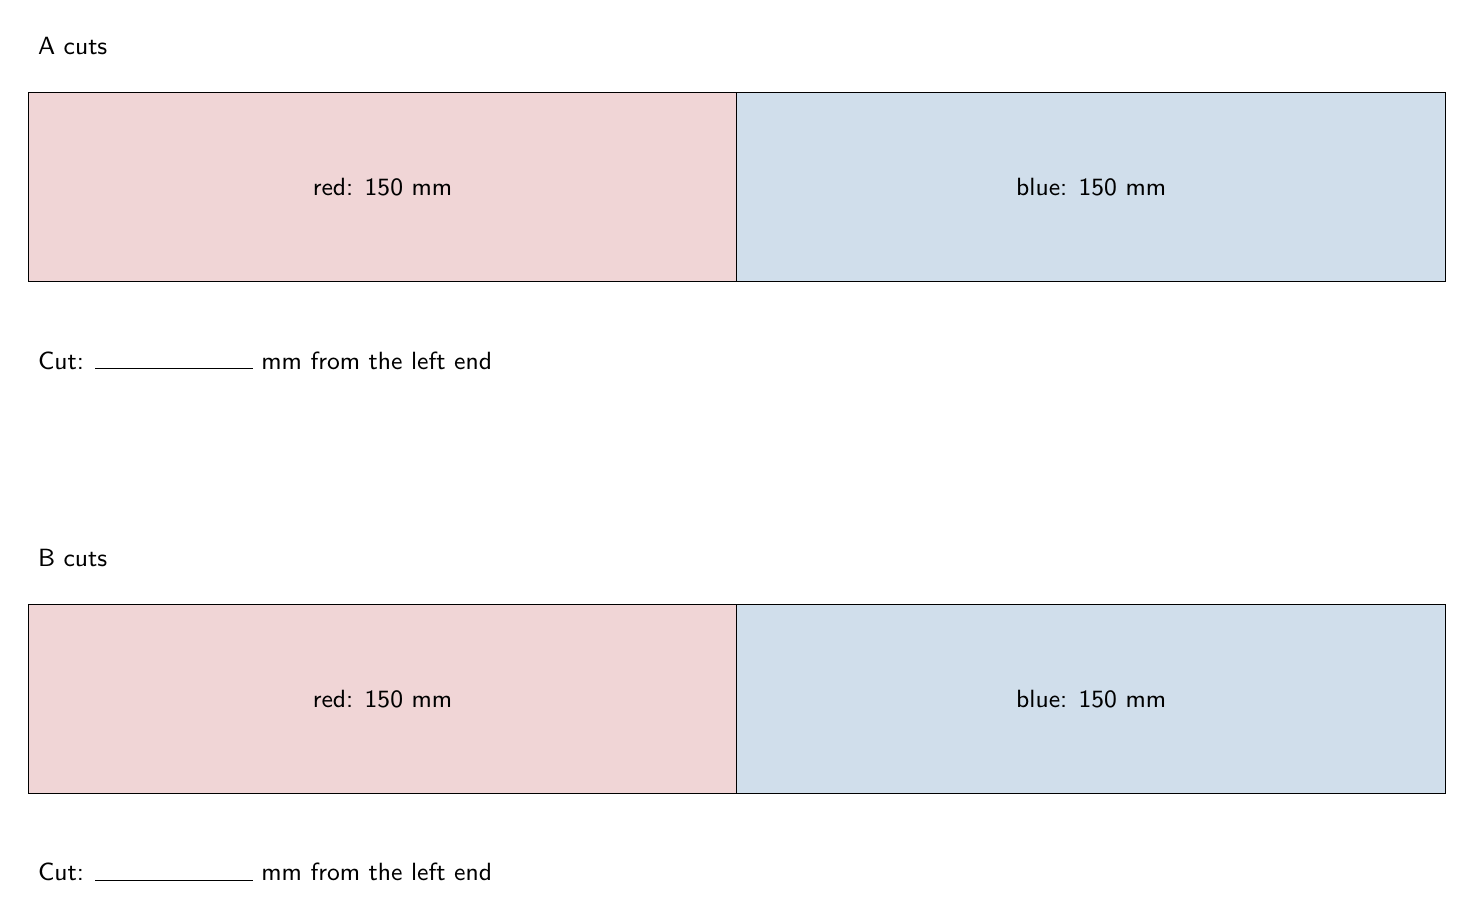
\begin{tikzpicture}[x=1mm,y=1mm]
  \node[anchor=west,font=\small] at (0,100){A cuts};\strip{0}{70}
  \node[anchor=west,font=\small] at (0,60){Cut: \rule{20mm}{.25pt}\ mm from the left end};
  \node[anchor=west,font=\small] at (0,35){B cuts};\strip{0}{5}
  \node[anchor=west,font=\small] at (0,-5){Cut: \rule{20mm}{.25pt}\ mm from the left end};
\end{tikzpicture}
\end{center}

\newband{Grades 3--5}
\prob{4}{Two people use a splittable strip. The cutter makes pieces of exactly equal value to the cutter. The chooser takes a piece they value at least as much as the other. Must both people receive at least half of their own total value? Must neither person envy the other? Explain.}

\linearea{6}

Both people now use A's strip preferences: a whole red panel is worth 3, and a whole blue panel is worth 1. The cutter cuts at the join between the colors. Does this cut-and-choose trial pass both checks?

\begin{center}
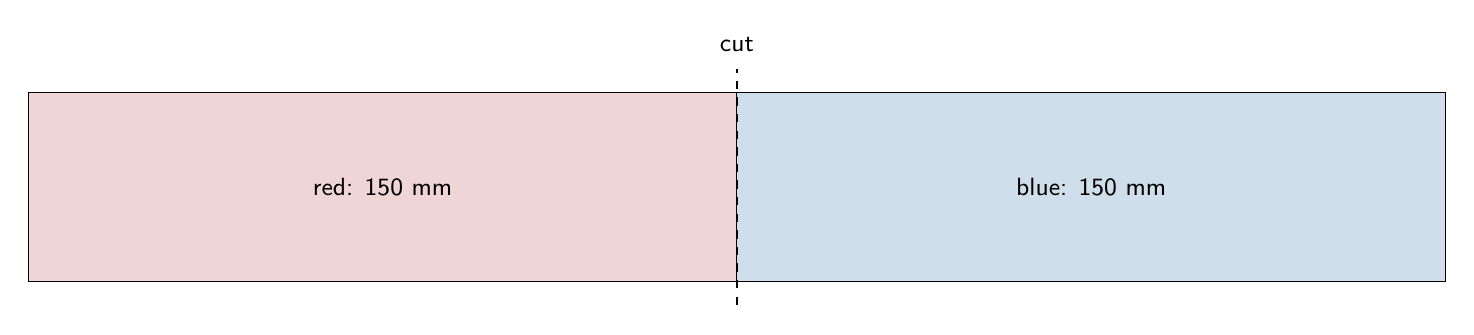
\begin{tikzpicture}[x=1mm,y=1mm]
  \strip{0}{2}
  \draw[dashed,line width=1pt] (90,-1) -- (90,29);
  \node[anchor=south,font=\small] at (90,30){cut};
\end{tikzpicture}
\end{center}
\linearea{4}

\newband{Grades 2--5}
\prob{5}{U and V each value every red card at 1. Divide all three cards between them, keeping each card whole, so neither person envies the other. If no division works, explain why. For a second trial, replace R3 with its paper copy; you may cut that copy. R1 and R2 must stay whole. Can you now make an envy-free division?}

\begin{center}
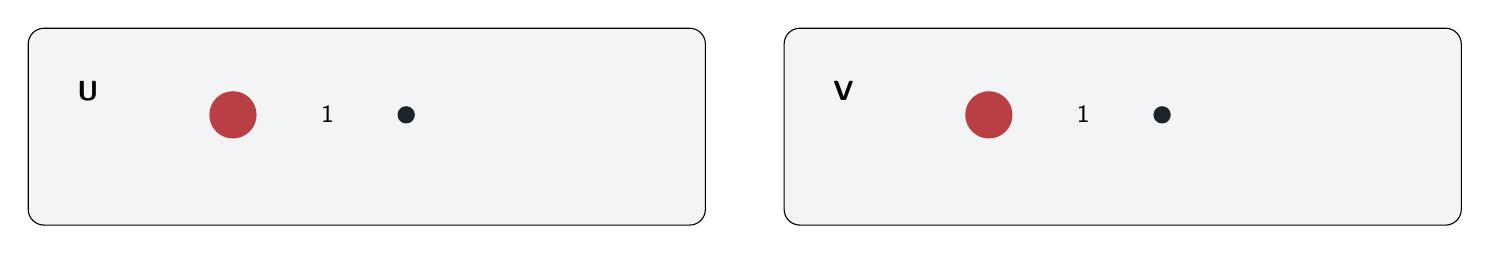
\begin{tikzpicture}[x=1mm,y=1mm]
  \foreach \x/\name in {0/U,96/V}{
    \draw[rounded corners=2mm,fill=pale] (\x,0) rectangle ++(86,25);
    \node[anchor=west,font=\bfseries] at (\x+5,17){\name};
    \fill[redgood] (\x+26,14) circle (3mm);
    \node[font=\small] at (\x+38,14){1};\valuedots{\x+44}{14}{1}
  }
\end{tikzpicture}
\end{center}
\begin{center}
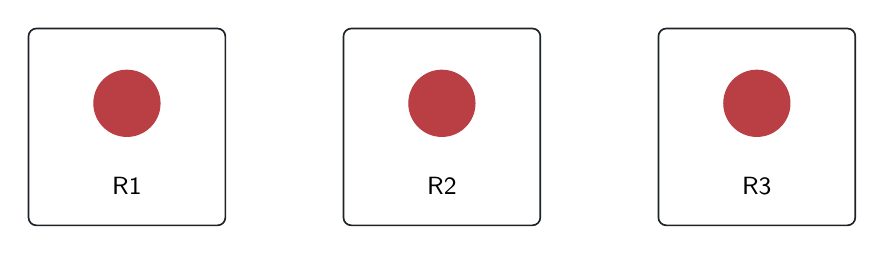
\begin{tikzpicture}[x=1mm,y=1mm]
  \good{38}{0}{1}{R1}\good{78}{0}{1}{R2}\good{118}{0}{1}{R3}
\end{tikzpicture}
\end{center}
In the second trial, R3's whole paper square is worth 1 to each person. Equal areas have equal value.

\begin{center}
\begin{tikzpicture}[x=1mm,y=1mm]
  \foreach \x/\label in {0/U,96/V}{
    \draw[rounded corners=3mm,black!40] (\x,0) rectangle ++(86,56);
    \node[anchor=north west,font=\small] at (\x+4,52){\label};
  }
\end{tikzpicture}
\end{center}
\linearea{5}

\newband{Grades 3--5}
For three people, proportional means each person's own tray is worth at least one third of everything, using their own values. Envy-free means their own tray is worth at least as much as \emph{each} other tray. Ties pass both checks.

\prob{6}{Use the three-person preference cards below with panels X, Y and Z. A receives X, B receives Y, and C receives Z. Is this division proportional for everyone? Is it envy-free for everyone? Rearrange the whole panels to make the division envy-free.}

\begin{center}
\renewcommand{\arraystretch}{1.8}
\begin{tabular}{|p{37mm}|>{\centering\arraybackslash}p{36mm}|>{\centering\arraybackslash}p{36mm}|>{\centering\arraybackslash}p{36mm}|}
\hline
Observer & X & Y & Z\\\hline
A & 4 & 8 & 0\\\hline
B & 0 & 4 & 8\\\hline
C & 8 & 0 & 4\\\hline
\end{tabular}
\end{center}
\begin{center}
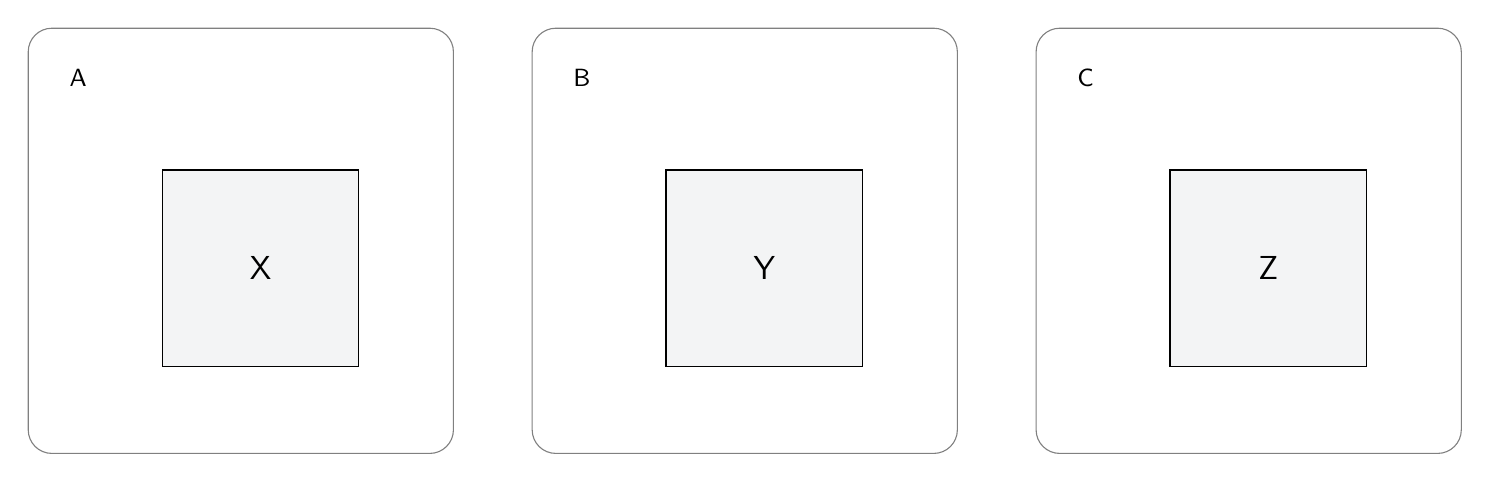
\begin{tikzpicture}[x=1mm,y=1mm]
  \foreach \x/\person/\panel in {0/A/X,64/B/Y,128/C/Z}{
    \draw[rounded corners=3mm,black!50] (\x,0) rectangle ++(54,54);
    \node[anchor=north west,font=\small] at (\x+4,50){\person};
    \draw[fill=pale] (\x+17,11) rectangle ++(25,25);
    \node[font=\large] at (\x+29.5,23.5){\panel};
  }
\end{tikzpicture}
\end{center}
\begin{center}
\renewcommand{\arraystretch}{1.65}
\begin{tabular}{|p{23mm}|p{31mm}|p{36mm}|p{36mm}|p{30mm}|}
\hline
\multicolumn{5}{|l|}{Initial allocation only: A has X, B has Y, C has Z}\\\hline
Observer & A's tray & B's tray & C's tray & One third of all\\\hline
A & & & &\\\hline
B & & & &\\\hline
C & & & &\\\hline
\end{tabular}
\end{center}
\linearea{3}

\newband{Grades 3--5}
\prob{7}{Every item goes to exactly one person, and tray values add. For two people, can a division be proportional but fail to be envy-free? Can it be envy-free but fail to be proportional? Explain your answers for any two-person division.}

\begin{center}
\begin{tikzpicture}[x=1mm,y=1mm]
  \node[anchor=west,font=\small] at (0,39){One observer's values};
  \draw[rounded corners=2mm] (0,0) rectangle (86,28);
  \draw[rounded corners=2mm] (96,0) rectangle (182,28);
  \node[font=\small] at (43,18){own tray};
  \node[font=\small] at (139,18){other tray};
\end{tikzpicture}
\end{center}
\linearea{4}

For three people, can a division be proportional but fail to be envy-free? Can it be envy-free but fail to be proportional? Give an example whenever the answer is yes, and explain why whenever the answer is no.

\begin{center}
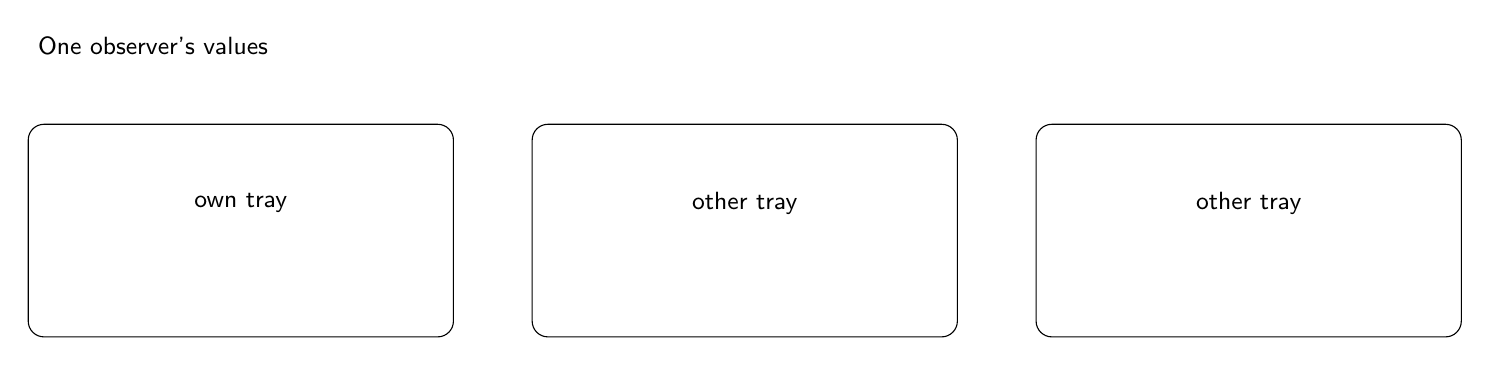
\begin{tikzpicture}[x=1mm,y=1mm]
  \node[anchor=west,font=\small] at (0,37){One observer's values};
  \foreach \x/\lab in {0/own tray,64/other tray,128/other tray}{
    \draw[rounded corners=2mm] (\x,0) rectangle ++(54,27);
    \node[font=\small] at (\x+27,17){\lab};
  }
\end{tikzpicture}
\end{center}
\linearea{3}

\end{document}
